\documentclass{article}
\usepackage[utf8]{inputenc}
\usepackage{amsmath}
\usepackage{graphicx}
\usepackage{caption}
\usepackage{float}

\title{Vergelijking Gauss-Legendre, Clenshaw-Curtis en Romberg
integratie}
\author{Alexander Boucquey, Peter Coppens, Simon Dirckx, Cedric Picron}
\date{}

\setlength\parindent{0pt}

\graphicspath{{./figs/}}

\begin{document}
\maketitle

\section{Exercise 1}

Figure~\ref{fig:f} contains a plot of all of the test functions.
We calculate the solutions of the integral analytically as:
\begin{equation}
\frac{1}{21} x^{21}, \quad e^x, \quad \frac{1}{2} \sqrt{\pi} \text{erf}(x),
\end{equation}
\begin{equation}
\frac{1}{4} tan^{-1}(4x), \quad \sqrt{\pi} \text{erf}(\frac{1}{x}) + e^{-\frac{1}{x^2}} x, \quad \frac{1}{4} x^4 \text{sign}(x)
\end{equation}

\begin{figure}[H]
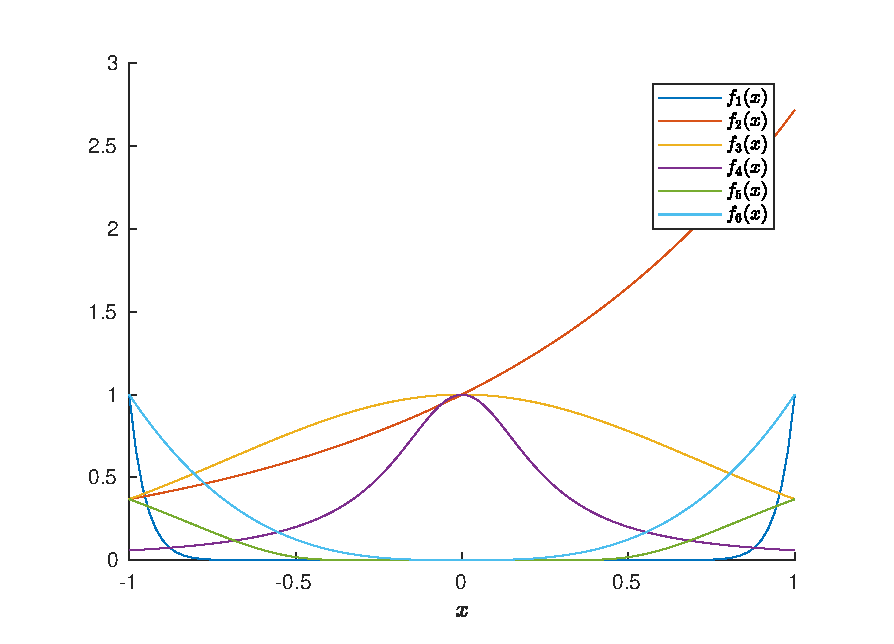
\includegraphics[width=0.7\linewidth]{f.eps}
\centering
\caption{The functions that we will be integrating.} \label{fig:f}
\end{figure}

\pagebreak
\section{Exercise 2}

We use the code provided in the paper as suggested. Calculating the analytical integral of $f_5(x)$ proved difficult, as the integral has a discontinuity in $x=0$. This is solved using the fact that the function is even, so we integrate over $\left[0, 1\right]$ and multiply the solution by $2$. \\

Figure~\ref{fig:re} shows the relative error. We notice that it is very similar to the solutions in the paper.

\begin{figure}[H]
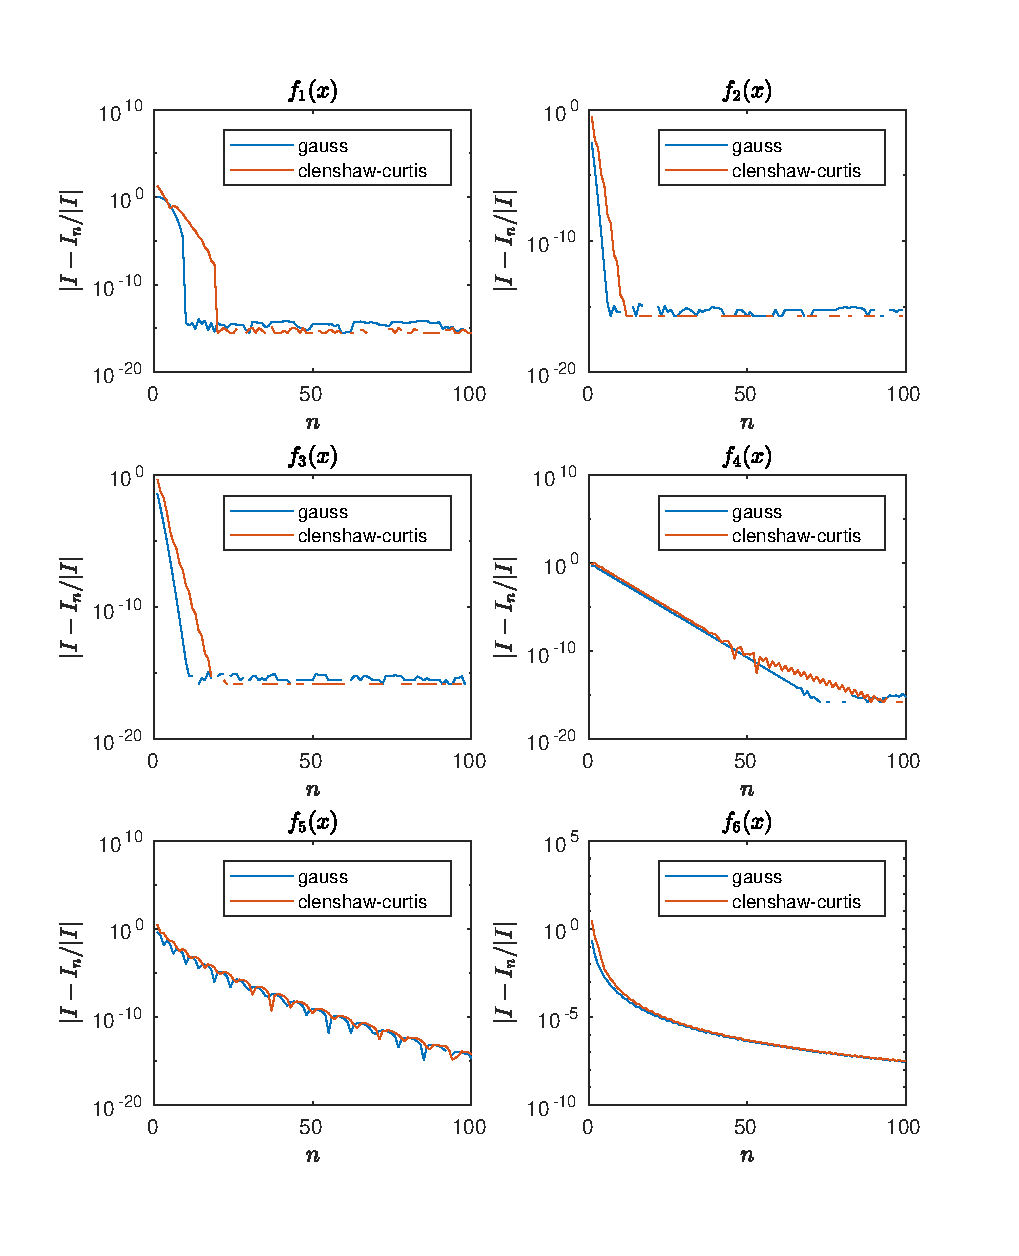
\includegraphics[width=0.9\linewidth]{re.eps}
\centering
\caption{The relative error for each function and each method.} \label{fig:re}
\end{figure}

\pagebreak

We also calculate the numerical cost to get to a precision of $7$ digits. \\
$f_1$: cost -- gauss: 10 -- clenshaw-curtis: 18 \\
$f_2$: cost -- gauss: 4  -- clenshaw-curtis: 6  \\
$f_3$: cost -- gauss: 6  -- clenshaw-curtis: 9  \\
$f_4$: cost -- gauss: 33 -- clenshaw-curtis: 35 \\
$f_5$: cost -- gauss: 34 -- clenshaw-curtis: 31 \\
$f_6$: cost -- gauss: 73 -- clenshaw-curtis: 75 \\
We notice that for $f_5$ clenshaw-curtis requires less points. For everything else clenshaw-curtis requires some more points, but only for $f_1$ it needs about twice as many. As predicted by the paper.

\end{document}
